\documentclass[xetex,mathserif,serif]{beamer}
\usepackage{polyglossia}
\setdefaultlanguage[babelshorthands=true]{russian}
\usepackage{minted}
\usepackage{tabu}

\usepackage{textpos}
\setlength{\TPHorizModule}{1cm}
\setlength{\TPVertModule}{1cm}

\useoutertheme{infolines}

\usepackage{fontspec}
\setmainfont{FreeSans}
\newfontfamily{\russianfonttt}{FreeSans}

\tabulinesep=0.7mm

\title{Проектирование распределённых приложений}
\subtitle{Часть вторая: высокоуровневые вещи}
\author[Юрий Литвинов]{Юрий Литвинов \newline \textcolor{gray}{\small\texttt{yurii.litvinov@gmail.com}}}

\date{14.12.2017}

\begin{document}
	
	\frame{\titlepage}

		\section{SOAP}

		\begin{frame}
		\frametitle{SOAP-ориентированные сервисы}
		\begin{columns}
			\begin{column}{0.6\textwidth}
				\begin{itemize}
					\item Simple Object Access Protocol
					\item Web Services Description Language
					\item Universal Discovery, Description and Integration
				\end{itemize}
			\end{column}
			\begin{column}{0.4\textwidth}
				\begin{center}
					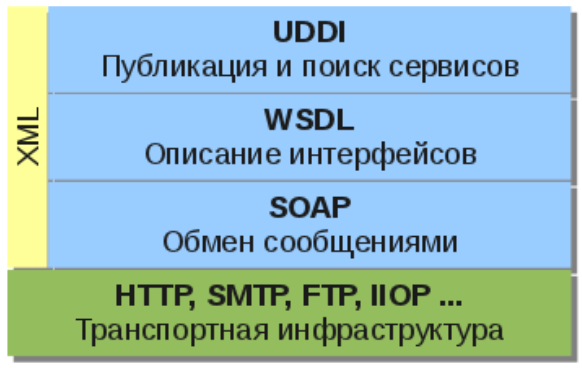
\includegraphics[width=\textwidth]{soap.png}
				\end{center}
			\end{column}
		\end{columns}
	\end{frame}

	\begin{frame}[fragile]
		\frametitle{SOAP-сообщение}
		\begin{small}
			\begin{minted}{xml}
<env:Envelope xmlns:env="http://www.w3.org/2003/05/soap-envelope">
    <env:Header>
        <n:alertcontrol xmlns:n="http://example.org/alertcontrol">
            <n:priority>1</n:priority>
            <n:expires>2001-06-22T14:00:00-05:00</n:expires>
        </n:alertcontrol>
    </env:Header>
    <env:Body>
        <m:alert xmlns:m="http://example.org/alert">
            <m:msg>Get up at 6:30 AM</m:msg>
        </m:alert>
    </env:Body>
</env:Envelope>
			\end{minted}
		\end{small}
	\end{frame}

	\begin{frame}
		\frametitle{Достоинства SOAP-based сервисов}
		\begin{itemize}
			\item Автоматический режим описания сервисов
			\item Автоматическая поддержка описаний SOAP-клиентом
			\item Автоматическая валидация сообщений
			\begin{itemize}
				\item Валидность xml
				\item Проверка по схеме
				\item Проверка SOAP-сервером
			\end{itemize}
			\item Работа через HTTP
			\begin{itemize}
				\item Хоть через обычный GET
			\end{itemize}
		\end{itemize}
	\end{frame}

	\begin{frame}
		\frametitle{Недостатки SOAP-based сервисов}
		\begin{itemize}
			\item Огромный размер сообщений
			\item Сложность описаний на клиенте и сервере
			\item Один запрос --- один ответ
			\begin{itemize}
				\item Поддержка транзакций на уровне бизнес-логики
			\end{itemize}
			\item Сложности миграции при изменении описания
		\end{itemize}
	\end{frame}

	\section{WCF}

	\begin{frame}
		\frametitle{Пример: WCF}
		\begin{itemize}
			\item Платформа для создания веб-сервисов
			\item Часть .NET Framework, начиная с 3.0
			\item Умеет WSDL, SOAP и т.д., очень конфигурируема
			\item Автоматическая генерация заглушек на стороне клиента
			\item ABCs of WCF:
			\begin{itemize}
				\item Address
				\item Binding
				\item Contract
			\end{itemize}
		\end{itemize}
		\begin{center}
			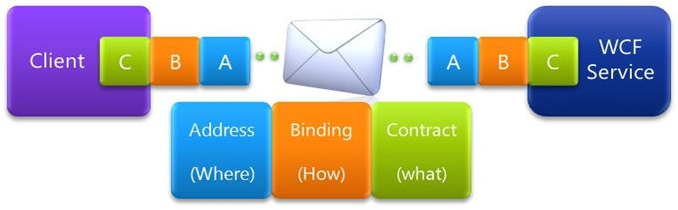
\includegraphics[width=0.6\textwidth]{wcf.png}
			\attribution{\url{http://www.c-sharpcorner.com}}
		\end{center}
	\end{frame}

	\begin{frame}[fragile]
		\frametitle{Пример, описание контракта}
		\begin{small}
			\begin{minted}{csharp}
[ServiceContract(Namespace = "http://Microsoft.ServiceModel.Samples")]  
public interface ICalculator  
{
    [OperationContract]
    double Add(double n1, double n2);

    [OperationContract]
    double Subtract(double n1, double n2);

    [OperationContract]
    double Multiply(double n1, double n2);

    [OperationContract]
    double Divide(double n1, double n2);
}
			\end{minted}
		\end{small}
	\end{frame}

	\begin{frame}[fragile]
		\frametitle{Пример, реализация контракта}
		\begin{small}
			\begin{minted}{csharp}
public class CalculatorService : ICalculator  
{
    public double Add(double n1, double n2)
        => n1 + n2;  

    public double Subtract(double n1, double n2)
        => n1 - n2

    public double Multiply(double n1, double n2)  
        => n1 * n2;

    public double Divide(double n1, double n2)  
        => n1 / n2;
}
			\end{minted}
		\end{small}
	\end{frame}

	\begin{frame}[fragile]
		\frametitle{Пример, self-hosted service}
		\begin{scriptsize}
			\begin{minted}{csharp}
static void Main(string[] args) 
{
    Uri baseAddress = new Uri("http://localhost:8000/ServiceModelSamples/Service");
    ServiceHost selfHost = new ServiceHost(typeof(CalculatorService), baseAddress);

    try {
        selfHost.AddServiceEndpoint(typeof(ICalculator), new WSHttpBinding(), "CalculatorService");

        ServiceMetadataBehavior smb = new ServiceMetadataBehavior();
        smb.HttpGetEnabled = true;
        selfHost.Description.Behaviors.Add(smb);

        selfHost.Open();
        Console.WriteLine("The service is ready. Press <ENTER> to terminate service.");
        Console.ReadLine();

        selfHost.Close();  
    } catch (CommunicationException ce) {
        Console.WriteLine($"An exception occurred: {ce.Message}");
        selfHost.Abort();
    }
}
			\end{minted}
		\end{scriptsize}
	\end{frame}

	\begin{frame}[fragile]
		\frametitle{Пример, клиент}
		\begin{itemize}
			\item Генерация заглушки: 
				\begin{scriptsize}
					\begin{minted}{text}
svcutil.exe /language:cs /out:generatedProxy.cs /config:app.config^
    http://localhost:8000/ServiceModelSamples/service
					\end{minted}
				\end{scriptsize}
			\item Клиент:
				\begin{footnotesize}
					\begin{minted}{csharp}
static void Main(string[] args)
{
    CalculatorClient client = new CalculatorClient();

    double value1 = 100.00D;
    double value2 = 15.99D;
    double result = client.Add(value1, value2);
    Console.WriteLine($"Add({value1},{value2}) = {result}");

    client.Close();
}
					\end{minted}
				\end{footnotesize}
		\end{itemize}
	\end{frame}

	\begin{frame}[fragile]
		\frametitle{Пример, конфигурация клиента}
		\begin{ssmall}
			\begin{minted}{xml}
<?xml version="1.0" encoding="utf-8" ?>  
<configuration>  
    <startup>   
      <!-- specifies the version of WCF to use-->  
        <supportedRuntime version="v4.0" sku=".NETFramework,Version=v4.5,Profile=Client" />  
    </startup>  
    <system.serviceModel>  
        <bindings>  
            <!-- Uses wsHttpBinding-->  
            <wsHttpBinding>  
                <binding name="WSHttpBinding_ICalculator" />  
            </wsHttpBinding>  
        </bindings>  
        <client>  
            <!-- specifies the endpoint to use when calling the service -->  
            <endpoint address="http://localhost:8000/ServiceModelSamples/Service/CalculatorService"  
                binding="wsHttpBinding" bindingConfiguration="WSHttpBinding_ICalculator"  
                contract="ServiceReference1.ICalculator" name="WSHttpBinding_ICalculator">  
                <identity>  
                    <userPrincipalName value="migree@redmond.corp.microsoft.com" />  
                </identity>  
            </endpoint>  
        </client>  
    </system.serviceModel>  
</configuration>
			\end{minted}
		\end{ssmall}
	\end{frame}

	\section{RabbitMQ}

	\begin{frame}
		\frametitle{RabbitMQ}
		\begin{itemize}
			\item Сервер и клиенты системы надёжной передачи сообщений
			\begin{itemize}
				\item Сообщение посылается на сервер и хранится там, пока его не заберут
				\item Продвинутые возможности по маршрутизации сообщений
			\end{itemize}
			\item Реализует протокол AMQP (Advanced Message Queuing Protocol), но может использовать и другие протоколы
			\item Сервер написан на Erlang, клиентские библиотеки доступны для практически чего угодно
		\end{itemize}
		\begin{textblock}{3}(8,0)
			
\includegraphics[width=\textwidth]{rabbitmqLogo.png}
		\end{textblock}
	\end{frame}

\end{document}
